\section{Part A}
\label{part_a}
In reinforcement learning there is no supervisor but a {\em reward} signal to guide the learning process. Even the feddback is delayed and not instantenous which sets it as a different paradigm from other machine learning methods. In a sequential decision making process an/the {\em agent} get to pick an action at every time step which tries to optimize the future cumulative {\em reward} signal.
Traditional Reinforcement Learning
requires explicit design of state space and action space, while the mapping from state space to action space is learned \cite{sutton1998introduction}.
 That makes the problem spaces and the possible states in an environment very limited, only with fully observable state of environment for agent.  Neural networks enhances RL with the capability to make the agent learn a state abstraction and a policy approximation directly from its input data in a partially observable environment. Deep RL is the fruitful outcome of this attempt of RL enhancement.

\subsection*{Formal RL Framework:}
The general RL problem is formalized as a discrete time stochastic
control process where an agent interacts with its environment in the
following way: the agent starts, in a given state within its environment
$s_0 \in \mathcal{S}$, by gathering an initial observation $\omega_0 \in \Omega$. At each time
step $t$, the agent has to take an action $a_t \in \mathcal{A}$. As illustrated in
Figure \ref{fig:rl_01} it follows three consequences: (i) the agent obtains a reward
$r_t \in \mathcal{R}$, (ii) the state transitions to $s_{t+1} \in \mathcal{S}$, and (iii) the agent obtains
an observation $\omega_{t+1} \in \Omega$. This control setting was first proposed by
\cite{bellman1957dynamic} and later extended to learning by Barto \cite{barto1983neuronlike}.
The goal of RL is to {\em select actions to maximise total future reward}.
\begin{figure}[t]
	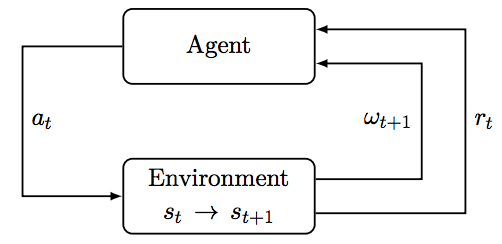
\includegraphics[width=0.7\linewidth ]{fig/agent.png}
    \vspace{-2mm}
    \caption{Agent-environment interaction in RL.}
    \label{fig:rl_01}
\end{figure}

\definition{\em Reward:}
A reward $r_t$ is a scalar feedback signal that indicates how well {\em agent} is doing at step $t$.

An example of  {\em reward} in the case of flying toy robot helicopters are : (a) $+$ve reward for following desired trajectory, (b) $−$ve reward for crashing.

\definition{\em History:} The history $\mathcal{H}_t$ is the sequence of observations, actions, rewards, i.e. all observable variables up to time $t$. Mathematically, $\mathcal{H}_t = \omega_1,r_1,a_1,\ldots,a_{t−1},\omega_t,r_t$.

Formally, state $s_t \in \mathcal{S}$ is a function of the history $\mathcal{H}_t$.
$$s_t = f(\mathcal{H}_t)$$

Environment and agent both can have threr own state which we define as $s_t^e$ and $s_t^a$ respectively. The environment state is usually not visible to the agent.

In a fully observable system, the agent directly observes environment state i.e. $\omega_t = s^a_t = s_t^e$. Formally this is called Markov Decision Process (MDP). The Markov property means that the future of the process only
depends on the current observation, and the agent has no interest in
looking at the full history.

\Paragraph{Markov Decision Process (MDP):}\\  An MDP is a 5-tuple $(\mathcal{S}, \mathcal{A}, T, \mathcal{R}, \gamma)$ where
\begin{itemize}
  \item[] $\mathcal{S}$ is the state space,
  \item[] $\mathcal{A}$ is the action space,
  \item[] $T : \mathcal{S} \times \mathcal{A}\times \mathcal{S} \rightarrow [0, 1]$ is the transition function (set of conditional
  transition probabilities between states),
  \item[] R: $\mathcal{S} \times \mathcal{A}\times \mathcal{S} \rightarrow \mathcal{R}$ is the reward function, where $R$ is a continuous set of possible rewards in a range $R_{max} \in \mathbb{R}^+$ (e.g., $[0, R_{max}]$),
  \item[] $\gamma \in  [0, 1)$ is the discount factor.
\end{itemize}

% $\mathcal{A}$ is the action space, \\
% $T : \mathcal{S} \times \mathcal{A}\times \mathcal{S} \rightarrow [0, 1]$ is the transition function (set of conditional
% transition probabilities between states), \\
% R: $\mathcal{S} \times \mathcal{A}\times \mathcal{S} \rightarrow \mathcal{R}$ is the reward function, where $R$ is a continuous set of possible rewards in a range $R_{max} \in \mathbb{R}^+$ (e.g., $[0, R_{max}]$), \\
% $\gamma \in  [0, 1)$ is the discount factor.

\vspace{3mm}

However, in the real world not many sytems are fully observable, an {\em agent} indirectly observes the environment without knowing it's internal information state. In this scenario $s_t^a \neq s^e_t$.

Formally this is a partially observable Markov decision process (POMDP).
\vspace{5mm}
\Paragraph{Partially Observable Markov Decision Process (POMDP):}
A POMDP is a 7-tuple $(\mathcal{S}, \mathcal{A}, T, \mathcal{R}, \Omega, O, \gamma)$ where
\begin{itemize}
  \item[] $\mathcal{S}$ is the state space,
  \item[] $\mathcal{A}$ is the action space,
  \item[] $T : \mathcal{S} \times \mathcal{A}\times \mathcal{S} \rightarrow [0, 1]$ is the transition function (set of conditional
  transition probabilities between states),
  \item[] R: $\mathcal{S} \times \mathcal{A}\times \mathcal{S} \rightarrow \mathcal{R}$ is the reward function, where $R$ is a continuous set of possible rewards in a range $R_{max} \in \mathbb{R}^+$ (e.g., $[0, R_{max}]$),
  \item[] $\Omega$ is a finite set of observations ${1, . . . , N_{\Omega}}$,
  \item[] $O : \mathcal{S} \times \Omega \rightarrow [0, 1]$ is a set of conditional observation probabilities,
  \item[] $\gamma \in  [0, 1)$ is the discount factor.
\end{itemize}


In a POMDP {\em agent} must construct its own state representation $s_t^a$. For example,\\
(i) \textbf{Complete history:} $s_t^a = \mathcal{H}_t$.\\
(ii) \textbf{{\em Beliefs} of environment state:} $s_t^a = \mathbb{P}[s_t^e = s^1],\ldots,\mathbb{P}[s_t^e = s^n]$ where $s^k$ represents a state in environment.\\
(iii) \textbf{Recurrent Neural Network (RNN)}: $s_t^a = \sigma(s_{t-1}^a W_s + \omega_t W_o)$ where $W_s$ and $W_o$ represents weight vectors and $\sigma$ some non linear function. \cite{wierstra2010recurrent, hausknecht2015deep, heess2015memory}.

This RNN approach to solving
POMDPs is related to other problems using dynamical systems
and state space models, where the true state can only be
estimated \cite{bertsekas2005dynamic}.


\subsection*{RL Agent Components:}
So far, we have introduced the key formalism used in RL,
the MDP and the POMDP. Now I will talk about what is inside an RL agent and the components it uses for learning. An RL agent may include one or more of these component for learning.\\
\Paragraph{\em Value functions:}
Value function attempts to measure goodness/badness of each state and/or action.
In other words, value function methods are based on estimating the value
(expected return) of being in a given state i.e. future reward.
The state-value
function $V_{\pi}(s)$
 is the expected return when starting in state $s$
and following $\pi$ henceforth:
$$V_{\pi}(s) = \mathbb{E}_\pi [R_t +\gamma R_{t+1} + \gamma^2 R_{t+2}+\ldots  | s_t =s ]$$
where $\gamma \in [0,1]$ is discount parameter, that governs the future sightedness of the model.
\\
\Paragraph{\em Policy Search:}  A policy is the {\em agent}'s behavior. It is a map from state to action. Examples of some policies are: \\
(i) {\em Deterministic Policy:} This is the simplest policy, here an action $a$ is mapped to a state $s$ i.e. $a = \pi(s)$.\\
(ii) {\em Stochastic Policy:} A policy can be stochastic based on probability of state observation, i.e. $\pi(a|s) = \mathbb{P}[\mathcal{A}=a |  \mathcal{S} = s]$.\\
(iii) {\em Parameterized Policy:} A parameterised policy $\pi_\theta$ is chosen, whose
parameters are updated to maximise the expected return $E[R|\theta]$ using either gradient-based or gradient-free optimisation \cite{deisenroth2013survey}. Neural networks that encode policies have been successfully
trained using both gradient-free \cite{gomez2005evolving, cuccu2011intrinsically, koutnik2013evolving} and gradient based \cite{williams1992simple, lillicrap2015continuous, heess2015learning} methods.

\Paragraph{\em Model:}
A model tries to learn the behavior of the environment. First, it tries to predict what the environment will do next, that is predicting next state and is called Transitions ($\mathcal{P}$). Secondly, the model tries to predict the expected next reward and is called Rewards model ($\mathcal{R}$).
$$\mathcal{P}^a_{ss'} = \mathbb{P}[\mathcal{S}' =s'| \mathcal{S}=s, \mathcal{A} =a]$$
where $s$ is the state prior state and $s'$ is the resultant state on action $a$.
$$\mathcal{R}^a_s = \mathbb{E}[r|\mathcal{S}=s,\mathcal{A}=a]$$
where $s$ is the state prior state and $r$ is the reward for next step on action $a$.

\subsection*{RL Agent Taxonomy:}
Model methods are optional in RL systems. In fact there are many model free based methods applied for real world problems. To understand a comprehensive taxonomies of categorizing RL Agent we present it in Figure \ref{fig:taxonomy}.

\begin{figure}[t]
	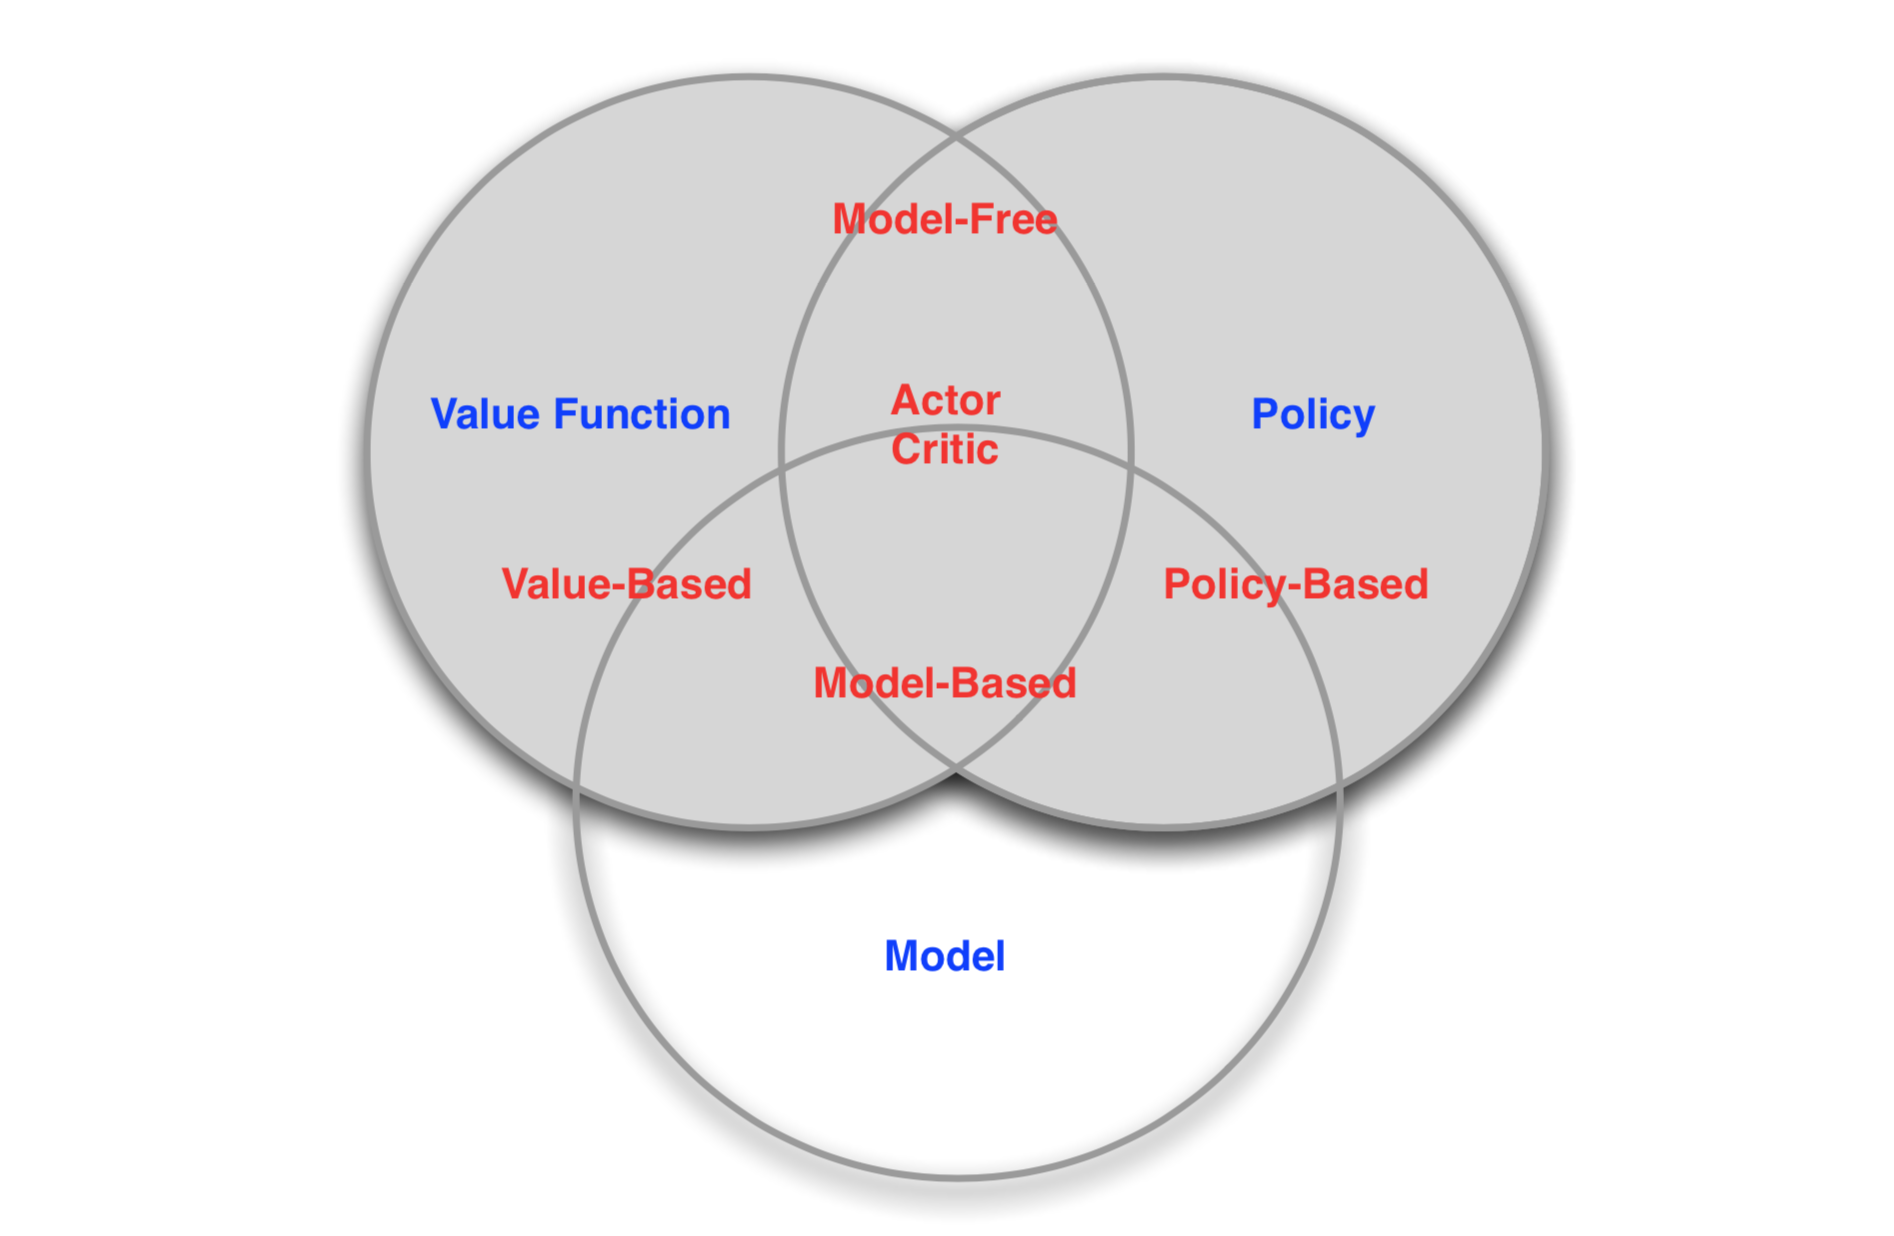
\includegraphics[width=0.7\linewidth ]{fig/taxonomy.png}
    \vspace{-2mm}
    \caption{RL Agent Taxonomy.}
    \label{fig:taxonomy}
\end{figure}

RL focus on learning without access to the underlying
model of the environment. However, interactions with the
environment could be used to learn value functions, policies,
and also a model. Model-free RL methods learn directly
from interactions with the environment, but model-based RL
methods can simulate transitions using the learned model,
resulting in increased sample efficiency \cite{arulkumaran2017brief}. This is particularly
important in domains where each interaction with the environment
is expensive. However, learning a model introduces extra
complexities, and there is always the danger of suffering from
model errors, which in turn affects the learned policy; a common
but partial solution in this latter scenario is to use model
predictive control, where planning is repeated after small
sequences of actions in the real environment \cite{bertsekas2005dynamic}.
Although
deep neural networks can potentially produce very complex
and rich models \cite{oh2015action, finn2016deep}, sometimes simpler, more data efficient
methods are preferable \cite{gu2016continuous}.

%%% Local Variables:
%%% mode: latex
%%% TeX-master: "main"
%%% End:
